\caption{step 1}
\label{Figure::inner_decision_step1}
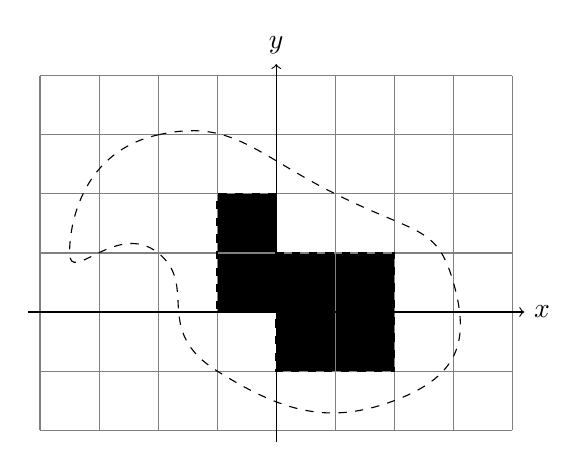
\begin{tikzpicture}[scale=0.75]
    % Define parameters
    \def\xmin{-4}
    \def\xmax{4}
    \def\ymin{-2}
    \def\ymax{4}

    % level 1
    \fill[\stepOneColor] (-1, 0) rectangle (0, 2);
    
    \fill[\stepOneColor]  (0, -1) rectangle (2, 1);
    
    \draw[step=1.0,gray,thin] (\xmin,\ymin) grid (\xmax,\ymax);

    % Axes
    \draw[->] (\xmin-0.2, 0) -- (\xmax+0.2, 0) node[right] {$x$};
    \draw[->] (0, \ymin-0.2) -- (0, \ymax+0.2) node[above] {$y$};
    
    \draw[dashed] plot [smooth cycle, tension=1] coordinates {(-3.5,1) (-2,3) (1,2) (3,0.5) (2,-1.5) (-1,-1)  (-2,1) };
    \draw[dashed, thick, black](-1,0) -- (0, 0) -- (0,-1) -- (2,-1) -- (2,1) -- (0,1) -- (0,2) -- (-1, 2) -- (-1,0);

\end{tikzpicture}
